% Options for packages loaded elsewhere
\PassOptionsToPackage{unicode}{hyperref}
\PassOptionsToPackage{hyphens}{url}
%
\documentclass[
]{book}
\usepackage{amsmath,amssymb}
\usepackage{iftex}
\ifPDFTeX
  \usepackage[T1]{fontenc}
  \usepackage[utf8]{inputenc}
  \usepackage{textcomp} % provide euro and other symbols
\else % if luatex or xetex
  \usepackage{unicode-math} % this also loads fontspec
  \defaultfontfeatures{Scale=MatchLowercase}
  \defaultfontfeatures[\rmfamily]{Ligatures=TeX,Scale=1}
\fi
\usepackage{lmodern}
\ifPDFTeX\else
  % xetex/luatex font selection
\fi
% Use upquote if available, for straight quotes in verbatim environments
\IfFileExists{upquote.sty}{\usepackage{upquote}}{}
\IfFileExists{microtype.sty}{% use microtype if available
  \usepackage[]{microtype}
  \UseMicrotypeSet[protrusion]{basicmath} % disable protrusion for tt fonts
}{}
\makeatletter
\@ifundefined{KOMAClassName}{% if non-KOMA class
  \IfFileExists{parskip.sty}{%
    \usepackage{parskip}
  }{% else
    \setlength{\parindent}{0pt}
    \setlength{\parskip}{6pt plus 2pt minus 1pt}}
}{% if KOMA class
  \KOMAoptions{parskip=half}}
\makeatother
\usepackage{xcolor}
\usepackage{color}
\usepackage{fancyvrb}
\newcommand{\VerbBar}{|}
\newcommand{\VERB}{\Verb[commandchars=\\\{\}]}
\DefineVerbatimEnvironment{Highlighting}{Verbatim}{commandchars=\\\{\}}
% Add ',fontsize=\small' for more characters per line
\usepackage{framed}
\definecolor{shadecolor}{RGB}{248,248,248}
\newenvironment{Shaded}{\begin{snugshade}}{\end{snugshade}}
\newcommand{\AlertTok}[1]{\textcolor[rgb]{0.94,0.16,0.16}{#1}}
\newcommand{\AnnotationTok}[1]{\textcolor[rgb]{0.56,0.35,0.01}{\textbf{\textit{#1}}}}
\newcommand{\AttributeTok}[1]{\textcolor[rgb]{0.13,0.29,0.53}{#1}}
\newcommand{\BaseNTok}[1]{\textcolor[rgb]{0.00,0.00,0.81}{#1}}
\newcommand{\BuiltInTok}[1]{#1}
\newcommand{\CharTok}[1]{\textcolor[rgb]{0.31,0.60,0.02}{#1}}
\newcommand{\CommentTok}[1]{\textcolor[rgb]{0.56,0.35,0.01}{\textit{#1}}}
\newcommand{\CommentVarTok}[1]{\textcolor[rgb]{0.56,0.35,0.01}{\textbf{\textit{#1}}}}
\newcommand{\ConstantTok}[1]{\textcolor[rgb]{0.56,0.35,0.01}{#1}}
\newcommand{\ControlFlowTok}[1]{\textcolor[rgb]{0.13,0.29,0.53}{\textbf{#1}}}
\newcommand{\DataTypeTok}[1]{\textcolor[rgb]{0.13,0.29,0.53}{#1}}
\newcommand{\DecValTok}[1]{\textcolor[rgb]{0.00,0.00,0.81}{#1}}
\newcommand{\DocumentationTok}[1]{\textcolor[rgb]{0.56,0.35,0.01}{\textbf{\textit{#1}}}}
\newcommand{\ErrorTok}[1]{\textcolor[rgb]{0.64,0.00,0.00}{\textbf{#1}}}
\newcommand{\ExtensionTok}[1]{#1}
\newcommand{\FloatTok}[1]{\textcolor[rgb]{0.00,0.00,0.81}{#1}}
\newcommand{\FunctionTok}[1]{\textcolor[rgb]{0.13,0.29,0.53}{\textbf{#1}}}
\newcommand{\ImportTok}[1]{#1}
\newcommand{\InformationTok}[1]{\textcolor[rgb]{0.56,0.35,0.01}{\textbf{\textit{#1}}}}
\newcommand{\KeywordTok}[1]{\textcolor[rgb]{0.13,0.29,0.53}{\textbf{#1}}}
\newcommand{\NormalTok}[1]{#1}
\newcommand{\OperatorTok}[1]{\textcolor[rgb]{0.81,0.36,0.00}{\textbf{#1}}}
\newcommand{\OtherTok}[1]{\textcolor[rgb]{0.56,0.35,0.01}{#1}}
\newcommand{\PreprocessorTok}[1]{\textcolor[rgb]{0.56,0.35,0.01}{\textit{#1}}}
\newcommand{\RegionMarkerTok}[1]{#1}
\newcommand{\SpecialCharTok}[1]{\textcolor[rgb]{0.81,0.36,0.00}{\textbf{#1}}}
\newcommand{\SpecialStringTok}[1]{\textcolor[rgb]{0.31,0.60,0.02}{#1}}
\newcommand{\StringTok}[1]{\textcolor[rgb]{0.31,0.60,0.02}{#1}}
\newcommand{\VariableTok}[1]{\textcolor[rgb]{0.00,0.00,0.00}{#1}}
\newcommand{\VerbatimStringTok}[1]{\textcolor[rgb]{0.31,0.60,0.02}{#1}}
\newcommand{\WarningTok}[1]{\textcolor[rgb]{0.56,0.35,0.01}{\textbf{\textit{#1}}}}
\usepackage{longtable,booktabs,array}
\usepackage{calc} % for calculating minipage widths
% Correct order of tables after \paragraph or \subparagraph
\usepackage{etoolbox}
\makeatletter
\patchcmd\longtable{\par}{\if@noskipsec\mbox{}\fi\par}{}{}
\makeatother
% Allow footnotes in longtable head/foot
\IfFileExists{footnotehyper.sty}{\usepackage{footnotehyper}}{\usepackage{footnote}}
\makesavenoteenv{longtable}
\usepackage{graphicx}
\makeatletter
\def\maxwidth{\ifdim\Gin@nat@width>\linewidth\linewidth\else\Gin@nat@width\fi}
\def\maxheight{\ifdim\Gin@nat@height>\textheight\textheight\else\Gin@nat@height\fi}
\makeatother
% Scale images if necessary, so that they will not overflow the page
% margins by default, and it is still possible to overwrite the defaults
% using explicit options in \includegraphics[width, height, ...]{}
\setkeys{Gin}{width=\maxwidth,height=\maxheight,keepaspectratio}
% Set default figure placement to htbp
\makeatletter
\def\fps@figure{htbp}
\makeatother
\setlength{\emergencystretch}{3em} % prevent overfull lines
\providecommand{\tightlist}{%
  \setlength{\itemsep}{0pt}\setlength{\parskip}{0pt}}
\setcounter{secnumdepth}{5}
\usepackage{booktabs}
\usepackage{booktabs}
\usepackage{longtable}
\usepackage{array}
\usepackage{multirow}
\usepackage{wrapfig}
\usepackage{float}
\usepackage{colortbl}
\usepackage{pdflscape}
\usepackage{tabu}
\usepackage{threeparttable}
\usepackage{threeparttablex}
\usepackage[normalem]{ulem}
\usepackage{makecell}
\usepackage{xcolor}
\ifLuaTeX
  \usepackage{selnolig}  % disable illegal ligatures
\fi
\usepackage[]{natbib}
\bibliographystyle{apalike}
\usepackage{bookmark}
\IfFileExists{xurl.sty}{\usepackage{xurl}}{} % add URL line breaks if available
\urlstyle{same}
\hypersetup{
  pdftitle={Example Analyses: Using the SGBA-5 with Simulated Data},
  pdfauthor={A Putman; S Dogra},
  hidelinks,
  pdfcreator={LaTeX via pandoc}}

\title{Example Analyses: Using the SGBA-5 with Simulated Data}
\author{A Putman \and S Dogra}
\date{2024-08-09}

\begin{document}
\maketitle

{
\setcounter{tocdepth}{1}
\tableofcontents
}
\chapter{About}\label{about}

The example analyses presented in this document are a demonstration of how sex-and gender-based analysis (SGBA) can be conducted using results from the Sex- and Gender-Based Analysis Tool -- 5 item (SGBA-5) by Putman and Dogra {[}DOI{]}.The examples in this document demonstrate a \hyperref[ux5cux23descriptive-analysis]{descriptive analysis} of simulated SGBA-5 responses and SGBA of simulated health outcomes that are \hyperref[continuous]{continuous}, ordered (Likert scale), or categorical (binary) to examine potential interactions with the biological sex item and two of the gendered aspects of health items.

The examples do not cover all potential analyses that could be done using the SGBA-5 but does provide a solid foundation from which researchers can select from and build upon.

\section{Further Resources}\label{further-resources}

More information on the SGBA-5, instructions for its use, and rationale for are included in the SGBA-5's documentation {[}SUPPLEMENTARY MATERIAL URL{]}. Initial reliability and validity testing of the SGBA-5 are reported in the paper by Putman, Cole, \& Dogra {[}DOI{]} and in A Putman's \href{https://ontariotechu.scholaris.ca/items/fddf2667-8cd6-429d-85bd-74b0076ab561}{thesis work}.

\chapter{Data Structure}\label{data-structure}

\section{Collected SGBA-5 Responses}\label{collected-sgba-5-responses}

After collecting responses from the SGBA-5 you will have a dataset that looks something like this:

\begin{verbatim}
## -- Attaching core tidyverse packages ------------------------ tidyverse 2.0.0 --
## v dplyr     1.1.4     v readr     2.1.5
## v forcats   1.0.0     v stringr   1.5.1
## v ggplot2   3.5.1     v tibble    3.2.1
## v lubridate 1.9.3     v tidyr     1.3.1
## v purrr     1.0.2     
## -- Conflicts ------------------------------------------ tidyverse_conflicts() --
## x dplyr::filter() masks stats::filter()
## x dplyr::lag()    masks stats::lag()
## i Use the conflicted package (<http://conflicted.r-lib.org/>) to force all conflicts to become errors
\end{verbatim}

\begin{table}

\caption{\label{tab:01-data}Example Data Structure}
\centering
\begin{tabular}[t]{rlrrrr}
\toprule
pt\_id & sex & gen\_id & gen\_exp & gen\_role & gen\_rel\\
\midrule
1 & Female & 48 & 99 & 70 & 25\\
2 & Male & 100 & 17 & 99 & 2\\
3 & Female & 64 & 48 & 88 & 40\\
4 & Female & 24 & 46 & 36 & 88\\
5 & Male & 73 & 23 & 19 & 26\\
\bottomrule
\multicolumn{6}{l}{\textsuperscript{} The values in this table are placeholders for the example, not real}\\
\multicolumn{6}{l}{data}\\
\end{tabular}
\end{table}

Where:

\texttt{pt\_id} is the participant identifier.

\texttt{sex} is the SGBA-5 categorical Biological Sex item.

\begin{itemize}
\tightlist
\item
  response options of ``male'', ``female'', and ``intersex''.
\end{itemize}

\texttt{gen\_id} is the SGBA-5 Gender Identity gendered aspect of health item.

\begin{itemize}
\tightlist
\item
  Responses are recorded as ordinal values between 0 to 100 on a feminine to masculine scale (measured in mm if completed on paper).
\end{itemize}

\texttt{gen\_exp} is the SGBA-5 Gender Expression gendered aspect of health item.

\begin{itemize}
\tightlist
\item
  Responses are recorded as ordinal values between 0 to 100 on a feminine to masculine scale (measured in mm if completed on paper).
\end{itemize}

\texttt{gen\_role} is the SGBA-5 Gender Role gendered aspect of health item.

\begin{itemize}
\tightlist
\item
  Responses are recorded as ordinal values between 0 to 100 on a feminine to masculine scale (measured in mm if completed on paper).
\end{itemize}

\texttt{gen\_rel} is the SGBA-5 Gender Relations gendered aspect of health item.

\begin{itemize}
\tightlist
\item
  Responses are recorded as ordinal values between 0 to 100 on a feminine to masculine scale (measured in mm if completed on paper).
\end{itemize}

\section{Simulated Data}\label{simulated-data}

This example analysis uses simulated data, if you wish to replicate the simulate data the code to do so is included in \href{}{Appendix A} or can be downloaded from this example's \href{https://github.com/putman-a/SGBA-5_example_analysis/\%s}{github page}.

\chapter{Descriptive Analysis}\label{descriptive-analysis}

\begin{quote}
\emph{Note: for conciseness, the following examples will only show results for two of the four gendered aspects of health items from the SGBA-5 (gender identity, and gender roles)}
\end{quote}

\section{Visualize Distribution of SGBA-5 Responses}\label{visualize-distribution-of-sgba-5-responses}

In plot \ref{fig:02-univar-sex-plot} we see that there are more participants who report their \textbf{biological sex} as assigned as female at birth (n=18) than males (n=12).

\begin{figure}

{\centering 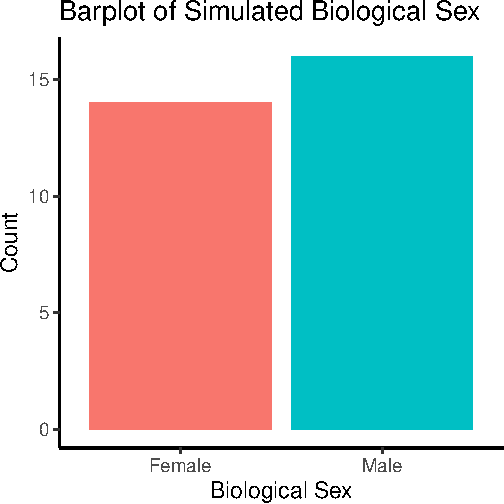
\includegraphics[width=0.5\linewidth]{02-descriptive-analysis_files/figure-latex/02-univar-sex-plot-1} 

}

\caption{Barplot of Biological Sex Responses}\label{fig:02-univar-sex-plot}
\end{figure}

Looking at the density plots for \textbf{gender identity} and \textbf{gender role} (figure \ref{fig:02-univar-gi-plot}), we see that while both variables are bimodal, the \textbf{gender identity} responses is more strongly bimodal with one peak closer to the feminine side of the feminine-masculine continuum and one peak closer to masculine end of that continuum. Further, we can also see that in general, participants reported their \textbf{gender identity} and \textbf{roles} as being more feminine, again with the \textbf{gender identity} responses showing this trend more strongly than the \textbf{gender role} responses.

\begin{figure}

{\centering 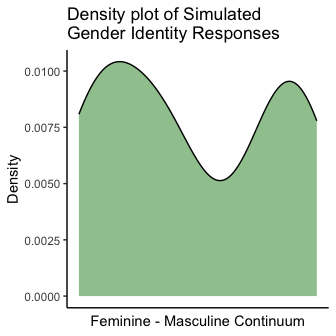
\includegraphics[width=0.5\linewidth]{02-descriptive-analysis_files/figure-latex/02-univar-gi-plot-1} 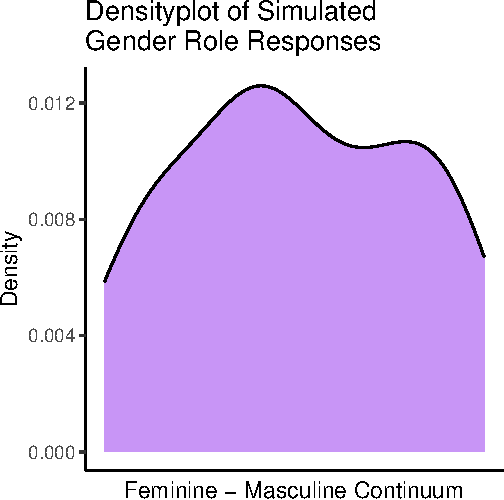
\includegraphics[width=0.5\linewidth]{02-descriptive-analysis_files/figure-latex/02-univar-gi-plot-2} 

}

\caption{Density plots of Gender Identity and Roles}\label{fig:02-univar-gi-plot}
\end{figure}

Presently, there is \emph{\textbf{no consensus on what descriptive statistics are most appropriate to report bimodal variables in health research}} (the typical mean(sd) or median(IQR) will not accurately represent that there is more than one peak in a bimodal variable's frequency distribution). When taken alongside the SGBA-5's assumption that the feminine-masculine continuum doesn't have a true 0 value, it is our suggestion that \emph{\textbf{if researchers decide to report a
single variable descriptive statistic for the gendered aspects of health item responses from the SGBA-5, they should provide a nominal description of skew}} along the feminine-masculine continuum as their descriptive statistic rather than the numerical average (or other summary statistic). To determine skew of one of the gender variables, the authors suggest calculating the sample's mean score along the feminine-masculine continuum and then classifying the skew using the classifications described in Table \ref{tab:02-tab}. Please note that these suggested classification guidelines are arbitrary and may not be appropriate in all circumstances.

\begin{table}

\caption{\label{tab:02-tab}Potential Interpretation of Sample Means for Gendered Aspect of Health Items.}
\centering
\begin{tabular}[t]{ll}
\toprule
Mean & Interpretation\\
\midrule
>70 & "Skews masculine"\\
55 to 70 & "More masculine than feminine"\\
45 to 55 & "Not strongly skewed"\\
30 to 45 & "More feminine than masculine"\\
<30 & "Skews feminine"\\
\bottomrule
\multicolumn{2}{l}{\textsuperscript{} This table assumes you have recorded the}\\
\multicolumn{2}{l}{gendered aspects of health items as 0}\\
\multicolumn{2}{l}{being the most feminine score and 100}\\
\multicolumn{2}{l}{being the most masculine score.}\\
\end{tabular}
\end{table}

For the simulated dataset represented in the density plots above, the mean score for the \textbf{gender identity} item was 50.2 and 46.8 for the \textbf{gender role} item. This means that when reporting descriptive statistics on the simulated sample we could report that: ``\emph{On the whole, the simulated
sample was not strongly skewed on a feminine to masculine continuum for either the gender identity or gender role measures from the SGBA-5}''.

Taking all these together, an example of a sample characteristics table of the SGBA-5 items in the simulated dataset could be presented as has been displayed in Table \ref{tab:02-tab02}

\begin{table}

\caption{\label{tab:02-tab02}Simulated sample characteristics.}
\centering
\begin{tabular}[t]{ll}
\toprule
SGBA Item & Sample (n = 30)\\
\midrule
Biological Sex (n(\%)) & \\
<i>Female</i> & 14(47\%)\\
<i>Intersex</i> & NA\\
<i>Male</i> & 16(53\%)\\
Gendered Aspect of Health (skew) & \\
\addlinespace
<i>Gender Identity</i> & Not strongly skewed\\
<i>Gendered Roles</i> & Not strongly skewed\\
\bottomrule
\end{tabular}
\end{table}

\chapter{SGBA of a Continuous Variable}\label{continuous}

\begin{quote}
\emph{Note: for conciseness, the following examples will only show results for two of the four gendered aspects of health items from the SGBA-5 (gender identity, and gender roles)}
\end{quote}

\section{Biological Sex}\label{biological-sex}

A good idea is to start by visualizing the continuous variable's distribution disaggregated by sex like the density plot in Figure \ref{fig:04-binary-pos-plot}. Then calculate disaggregated summary statistics for the continuous variable disaggregated by sex (Table A4), and conduct a statistical test of difference in means (Welch's t- test for this example).

\subsection{Density Plot}\label{density-plot}

\emph{Interpretation:} From the above density plots (Figure \ref{fig:04-binary-pos-plot}) we can see a distinct overlap in the \emph{``No interaction example''} with suggests that in that example's sample does not have a meaningful difference in the continuous outcome by sex. Conversely, the \emph{``Interaction example''} density plot has two distinct peaks which suggests that its sample's continuous outcome scores are associated with a participant's sex.

\begin{figure}

{\centering 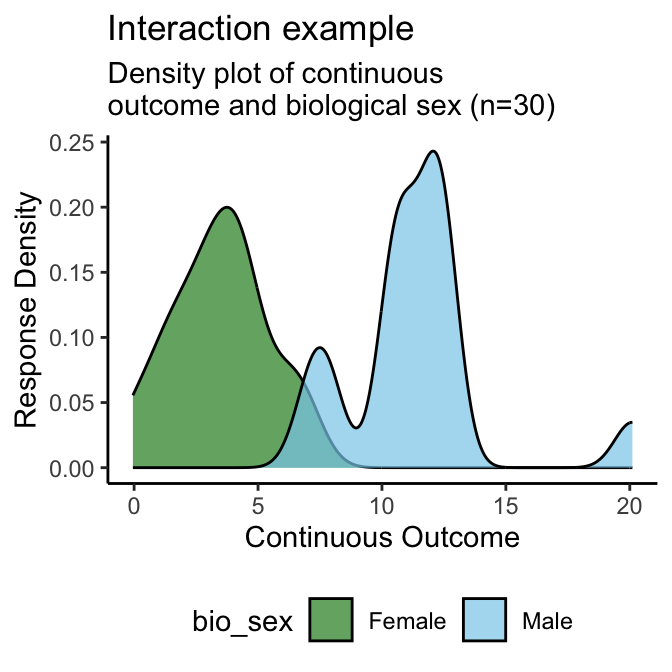
\includegraphics[width=0.5\linewidth]{03-continuous_files/figure-latex/04-binary-pos-plot-1} 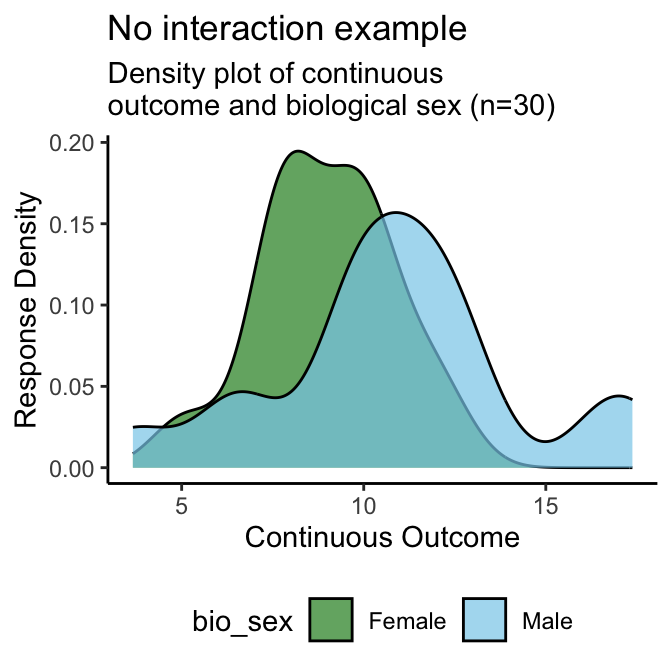
\includegraphics[width=0.5\linewidth]{03-continuous_files/figure-latex/04-binary-pos-plot-2} 

}

\caption{Density Plot of Continuous Variable by Biological Sex Examples}\label{fig:04-binary-pos-plot}
\end{figure}

\subsection{Summary Statistics}\label{summary-statistics}

\emph{Interpretation:} As with the density plots, we see that the standard deviations of the continuous variable for both males and females overlap in the \emph{``No interaction example''} (Table \ref{tab:03-tab-int}) - indicating a lack of significant difference by sex. The standard deviations of the continuous variable for both males and females do not overlap in the \emph{``Interaction example''} (Table \ref{tab:03-tab-no-int}) - indicating a potential association between the continuous outcome and sex.

\begin{table}

\caption{\label{tab:03-tab-int}Interation example summary statisitics: Continuous outcome and biological sex}
\centering
\begin{tabular}[t]{lrrrrr}
\toprule
biological sex & n & mean continuous & SD continuous & median continuous & IQR continuous\\
\midrule
Female & 14 & 3.5 & 1.94 & 4 & 2\\
Male & 16 & 11.3 & 2.95 & 11 & 2\\
\bottomrule
\end{tabular}
\end{table}

\begin{table}

\caption{\label{tab:03-tab-no-int}No interation example summary statisitics: Continuous outcome and biological sex}
\centering
\begin{tabular}[t]{lrrrrr}
\toprule
biological sex & n & mean continuous & SD continuous & median continuous & IQR continuous\\
\midrule
Female & 14 & 9.0 & 1.84 & 9 & 2\\
Male & 16 & 10.8 & 3.47 & 11 & 3\\
\bottomrule
\end{tabular}
\end{table}

\subsection{Statistical Test}\label{statistical-test}

\textbf{No interaction: Welch's t-test}

\begin{table}

\caption{\label{tab:unnamed-chunk-1}Simulated sample characteristics.}
\centering
\begin{tabular}[t]{llrlrr}
\toprule
Example & Test & T-score & 95\% CI & df & p-value\\
\midrule
Interaction & Welch's t-test & -1.80 & (-3.85, 0.26) & 23.4 & 0.084\\
No interaction & Welch's t-test & -8.73 & (-9.72, -6.02) & 26.1 & 0.000\\
\bottomrule
\end{tabular}
\end{table}

\chapter*{Appendix}\label{appendix}
\addcontentsline{toc}{chapter}{Appendix}

\section{Simulated Data Creation}\label{simulated-data-creation}

Below is the code used to create the simulated data that will be used to create the example SGBA seen throughout the rest of this example analysis.

\begin{Shaded}
\begin{Highlighting}[]
\CommentTok{\# load libraries {-}{-}{-}{-}{-}{-}{-}{-}{-}{-}{-}{-}{-}{-}{-}{-}{-}{-}{-}{-}{-}{-}{-}{-}{-}{-}{-}{-}{-}{-}{-}{-}{-}{-}{-}{-}{-}{-}{-}{-}{-}{-}{-}{-}{-}{-}{-}{-}{-}{-}{-}{-}{-}{-}{-}{-}{-}{-}}
\FunctionTok{library}\NormalTok{(tidyverse)}
\end{Highlighting}
\end{Shaded}

\begin{verbatim}
## -- Attaching core tidyverse packages ------------------------ tidyverse 2.0.0 --
## v dplyr     1.1.4     v readr     2.1.5
## v forcats   1.0.0     v stringr   1.5.1
## v ggplot2   3.5.1     v tibble    3.2.1
## v lubridate 1.9.3     v tidyr     1.3.1
## v purrr     1.0.2     
## -- Conflicts ------------------------------------------ tidyverse_conflicts() --
## x dplyr::filter() masks stats::filter()
## x dplyr::lag()    masks stats::lag()
## i Use the conflicted package (<http://conflicted.r-lib.org/>) to force all conflicts to become errors
\end{verbatim}

\begin{Shaded}
\begin{Highlighting}[]
\CommentTok{\# set seed for predictability}
\FunctionTok{set.seed}\NormalTok{(}\DecValTok{42}\NormalTok{, }\AttributeTok{kind =} \StringTok{"Mersenne{-}Twister"}\NormalTok{)}

\CommentTok{\# write simulation functions {-}{-}{-}{-}{-}{-}{-}{-}{-}{-}{-}{-}{-}{-}{-}{-}{-}{-}{-}{-}{-}{-}{-}{-}{-}{-}{-}{-}{-}{-}{-}{-}{-}{-}{-}{-}{-}{-}{-}{-}{-}{-}{-}{-}{-}{-}}

\CommentTok{\# function for simulating bimodal gender variables}
\NormalTok{binom\_bounded }\OtherTok{\textless{}{-}} \ControlFlowTok{function}\NormalTok{(}
\NormalTok{    n, prop, mean1, sd1, mean2, sd2, }\AttributeTok{lim\_low =} \SpecialCharTok{{-}}\ConstantTok{Inf}\NormalTok{, }\AttributeTok{lim\_up =} \ConstantTok{Inf}\NormalTok{, round}
\NormalTok{    )\{}
  \CommentTok{\# error checking}
  \ControlFlowTok{if}\NormalTok{(prop }\SpecialCharTok{\textgreater{}} \DecValTok{1} \SpecialCharTok{||}\NormalTok{ prop}\SpecialCharTok{\textless{}} \DecValTok{0}\NormalTok{)\{}\FunctionTok{stop}\NormalTok{(}\StringTok{"binomial proportion should be between 0 and 1"}\NormalTok{)\}}
  \ControlFlowTok{if}\NormalTok{(n }\SpecialCharTok{\textless{}} \DecValTok{1}\NormalTok{)\{}\FunctionTok{stop}\NormalTok{(}\StringTok{"n must be greater than or equal to 1"}\NormalTok{)\}}
  \ControlFlowTok{if}\NormalTok{(sd1 }\SpecialCharTok{\textless{}} \DecValTok{0} \SpecialCharTok{||}\NormalTok{ sd2 }\SpecialCharTok{\textless{}} \DecValTok{0}\NormalTok{)\{}\FunctionTok{stop}\NormalTok{(}\StringTok{"standard deviations must be non{-}negative"}\NormalTok{)\}}
  \CommentTok{\# create index}
\NormalTok{  index }\OtherTok{\textless{}{-}} \FunctionTok{rbinom}\NormalTok{(n, }\AttributeTok{size =} \DecValTok{1}\NormalTok{, }\AttributeTok{prob =}\NormalTok{ prop)}
  \CommentTok{\# simulate each peak using a bounded \textasciigrave{}rnorm()\textasciigrave{}}
\NormalTok{  binom\_sim1 }\OtherTok{\textless{}{-}}\NormalTok{ index }\SpecialCharTok{*} \FunctionTok{qnorm}\NormalTok{(}
    \FunctionTok{runif}\NormalTok{(}
\NormalTok{      n, }\FunctionTok{pnorm}\NormalTok{(lim\_low, mean1, sd1), }\FunctionTok{pnorm}\NormalTok{(lim\_up, mean1, sd1)}
\NormalTok{      ), }
\NormalTok{    mean1, sd1)}
\NormalTok{  binom\_sim0 }\OtherTok{\textless{}{-}}\NormalTok{ (}\DecValTok{1} \SpecialCharTok{{-}}\NormalTok{ index) }\SpecialCharTok{*} \FunctionTok{qnorm}\NormalTok{(}
    \FunctionTok{runif}\NormalTok{(}
\NormalTok{      n, }\FunctionTok{pnorm}\NormalTok{(lim\_low, mean2, sd2), }\FunctionTok{pnorm}\NormalTok{(lim\_up, mean2, sd2)}
\NormalTok{      ), }
\NormalTok{    mean2, sd2)}
\NormalTok{  binom\_sim }\OtherTok{\textless{}{-}}\NormalTok{ binom\_sim0 }\SpecialCharTok{+}\NormalTok{ binom\_sim1}
\NormalTok{  binom\_sim }\OtherTok{\textless{}{-}} \FunctionTok{round}\NormalTok{(binom\_sim, round)}
\NormalTok{  binom\_sim}
\NormalTok{\}}


\CommentTok{\# function for simulating Likert/ordinal outcome variable}
\NormalTok{ordinal\_sim }\OtherTok{\textless{}{-}} \ControlFlowTok{function}\NormalTok{(}
\NormalTok{    n, mean, sd, }\AttributeTok{lim\_low =} \SpecialCharTok{{-}}\ConstantTok{Inf}\NormalTok{, }\AttributeTok{lim\_up =} \ConstantTok{Inf}
\NormalTok{    )\{}
\NormalTok{  ord\_sim }\OtherTok{\textless{}{-}} \FunctionTok{qnorm}\NormalTok{(}
    \FunctionTok{runif}\NormalTok{(}
\NormalTok{      n, }\FunctionTok{pnorm}\NormalTok{(lim\_low, mean, sd), }\FunctionTok{pnorm}\NormalTok{(lim\_up, mean, sd)}
\NormalTok{      ),}
\NormalTok{    mean, sd)}
\NormalTok{  ord\_sim }\OtherTok{\textless{}{-}} \FunctionTok{round}\NormalTok{(ord\_sim, }\DecValTok{0}\NormalTok{)}
\NormalTok{  ord\_sim}
\NormalTok{\}}


\CommentTok{\# simulate SGBA{-}5 data with n of 30 {-}{-}{-}{-}{-}{-}{-}{-}{-}{-}{-}{-}{-}{-}{-}{-}{-}{-}{-}{-}{-}{-}{-}{-}{-}{-}{-}{-}{-}{-}{-}{-}{-}{-}{-}{-}{-}}

\CommentTok{\# biological sex: categorical (female, intersex, male)}
\NormalTok{bio\_sex }\OtherTok{\textless{}{-}} \FunctionTok{factor}\NormalTok{(}
  \FunctionTok{sample}\NormalTok{(}\FunctionTok{c}\NormalTok{(}\StringTok{\textquotesingle{}Female\textquotesingle{}}\NormalTok{, }\StringTok{\textquotesingle{}Male\textquotesingle{}}\NormalTok{), }\DecValTok{30}\NormalTok{, }\AttributeTok{replace=}\ConstantTok{TRUE}\NormalTok{, }\AttributeTok{prob=}\FunctionTok{c}\NormalTok{(}\FloatTok{0.6}\NormalTok{, }\FloatTok{0.4}\NormalTok{)),}
\NormalTok{  )}

\CommentTok{\# gender identity: ordered (0 [feminine] to 100 [masculine])}
\NormalTok{gen\_id }\OtherTok{\textless{}{-}} \FunctionTok{binom\_bounded}\NormalTok{(}
  \AttributeTok{n =} \DecValTok{30}\NormalTok{, }\AttributeTok{prop =} \FloatTok{0.6}\NormalTok{, }\AttributeTok{mean1 =} \DecValTok{20}\NormalTok{, }\AttributeTok{sd1 =} \DecValTok{20}\NormalTok{, }\AttributeTok{mean2 =} \DecValTok{85}\NormalTok{, }\AttributeTok{sd2 =} \DecValTok{15}\NormalTok{, }\AttributeTok{lim\_low =} \DecValTok{0}\NormalTok{,}
  \AttributeTok{lim\_up =} \DecValTok{100}\NormalTok{, }\AttributeTok{round =} \DecValTok{0}
\NormalTok{)}

\CommentTok{\# gender role: ordered (0 [feminine] to 100 [masculine])}
\NormalTok{gen\_role }\OtherTok{\textless{}{-}} \FunctionTok{binom\_bounded}\NormalTok{(}
  \AttributeTok{n =} \DecValTok{30}\NormalTok{, }\AttributeTok{prop =} \FloatTok{0.6}\NormalTok{, }\AttributeTok{mean1 =} \DecValTok{25}\NormalTok{, }\AttributeTok{sd1 =} \DecValTok{20}\NormalTok{, }\AttributeTok{mean2 =} \DecValTok{80}\NormalTok{, }\AttributeTok{sd2 =} \DecValTok{20}\NormalTok{, }\AttributeTok{lim\_low =} \DecValTok{0}\NormalTok{,}
  \AttributeTok{lim\_up =} \DecValTok{100}\NormalTok{, }\AttributeTok{round =} \DecValTok{0}
\NormalTok{)}


\CommentTok{\# simulate example positive outcome data with n of 30 {-}{-}{-}{-}{-}{-}{-}{-}{-}{-}{-}{-}{-}{-}{-}{-}{-}{-}{-}{-}{-}{-}{-}}

\DocumentationTok{\#\# simulated numerical outcome: {-}{-}{-}{-}{-}{-}{-}{-}{-}{-}{-}{-}{-}{-}{-}{-}{-}{-}{-}{-}{-}{-}{-}{-}{-}{-}{-}{-}{-}{-}{-}{-}{-}{-}{-}{-}{-}{-}{-}{-}{-}{-}{-}{-}}

\CommentTok{\# by sex: males (mean = 12, SD = 3), females (mean = 4, sd = 2)}
\NormalTok{outcome\_num\_pos\_m }\OtherTok{\textless{}{-}} \FunctionTok{rnorm}\NormalTok{(}\AttributeTok{n =} \DecValTok{16}\NormalTok{, }\AttributeTok{mean =} \DecValTok{12}\NormalTok{, }\AttributeTok{sd =} \DecValTok{3}\NormalTok{)}
\NormalTok{outcome\_num\_pos\_f }\OtherTok{\textless{}{-}} \FunctionTok{rnorm}\NormalTok{(}\AttributeTok{n =} \DecValTok{14}\NormalTok{, }\AttributeTok{mean =} \DecValTok{4}\NormalTok{, }\AttributeTok{sd =} \DecValTok{2}\NormalTok{)}
\NormalTok{outcome\_num\_pos\_sex }\OtherTok{\textless{}{-}} \FunctionTok{c}\NormalTok{(outcome\_num\_pos\_f, outcome\_num\_pos\_m)}

\CommentTok{\# by g\_id: high (mean = 12, SD = 3), low (mean = 4, sd = 2)}
\NormalTok{outcome\_num\_pos\_gid\_high }\OtherTok{\textless{}{-}} \FunctionTok{rnorm}\NormalTok{(}\AttributeTok{n =} \DecValTok{15}\NormalTok{, }\AttributeTok{mean =} \DecValTok{12}\NormalTok{, }\AttributeTok{sd =} \DecValTok{3}\NormalTok{)}
\NormalTok{outcome\_num\_pos\_gid\_low }\OtherTok{\textless{}{-}} \FunctionTok{rnorm}\NormalTok{(}\AttributeTok{n =} \DecValTok{15}\NormalTok{, }\AttributeTok{mean =} \DecValTok{4}\NormalTok{, }\AttributeTok{sd =} \DecValTok{2}\NormalTok{)}
\NormalTok{outcome\_num\_pos\_gid }\OtherTok{\textless{}{-}} \FunctionTok{c}\NormalTok{(outcome\_num\_pos\_gid\_high, outcome\_num\_pos\_gid\_low)}

\CommentTok{\# by g\_role: high (mean = 12, SD = 3), low (mean = 4, sd = 2)}
\NormalTok{outcome\_num\_pos\_grol\_high }\OtherTok{\textless{}{-}} \FunctionTok{rnorm}\NormalTok{(}\AttributeTok{n =} \DecValTok{12}\NormalTok{, }\AttributeTok{mean =} \DecValTok{12}\NormalTok{, }\AttributeTok{sd =} \DecValTok{3}\NormalTok{)}
\NormalTok{outcome\_num\_pos\_grol\_low }\OtherTok{\textless{}{-}} \FunctionTok{rnorm}\NormalTok{(}\AttributeTok{n =} \DecValTok{18}\NormalTok{, }\AttributeTok{mean =} \DecValTok{7}\NormalTok{, }\AttributeTok{sd =} \DecValTok{2}\NormalTok{)}
\NormalTok{outcome\_num\_pos\_grol }\OtherTok{\textless{}{-}} \FunctionTok{c}\NormalTok{(outcome\_num\_pos\_grol\_high, outcome\_num\_pos\_grol\_low)}


\DocumentationTok{\#\# simulated Likert outcome: {-}{-}{-}{-}{-}{-}{-}{-}{-}{-}{-}{-}{-}{-}{-}{-}{-}{-}{-}{-}{-}{-}{-}{-}{-}{-}{-}{-}{-}{-}{-}{-}{-}{-}{-}{-}{-}{-}{-}{-}{-}{-}{-}{-}{-}}

\CommentTok{\# by sex males (mean = 2, SD = 1), females (mean = 5, sd = 2)}
\NormalTok{outcome\_ord\_pos\_m }\OtherTok{\textless{}{-}} \FunctionTok{ordinal\_sim}\NormalTok{(}
  \AttributeTok{n =} \DecValTok{16}\NormalTok{, }\AttributeTok{mean =} \DecValTok{2}\NormalTok{, }\AttributeTok{sd =} \DecValTok{1}\NormalTok{, }\AttributeTok{lim\_low =} \DecValTok{1}\NormalTok{, }\AttributeTok{lim\_up =} \DecValTok{7}
\NormalTok{)}
\NormalTok{outcome\_ord\_pos\_f }\OtherTok{\textless{}{-}} \FunctionTok{ordinal\_sim}\NormalTok{(}
  \AttributeTok{n =} \DecValTok{14}\NormalTok{, }\AttributeTok{mean =} \DecValTok{5}\NormalTok{, }\AttributeTok{sd =} \DecValTok{1}\NormalTok{, }\AttributeTok{lim\_low =} \DecValTok{1}\NormalTok{, }\AttributeTok{lim\_up =} \DecValTok{7}
\NormalTok{)}
\NormalTok{outcome\_ord\_pos\_sex }\OtherTok{\textless{}{-}} \FunctionTok{c}\NormalTok{(outcome\_ord\_pos\_f, outcome\_ord\_pos\_m) }\SpecialCharTok{\%\textgreater{}\%}
  \FunctionTok{factor}\NormalTok{(., }\AttributeTok{levels =} \FunctionTok{c}\NormalTok{(}\DecValTok{1}\NormalTok{,}\DecValTok{2}\NormalTok{,}\DecValTok{3}\NormalTok{,}\DecValTok{4}\NormalTok{,}\DecValTok{5}\NormalTok{,}\DecValTok{6}\NormalTok{,}\DecValTok{7}\NormalTok{), }\AttributeTok{ordered =} \ConstantTok{TRUE}\NormalTok{)}


\CommentTok{\# by g\_id: high (mean = 5, SD = 2), low (mean = 1, sd = 2)}
\NormalTok{outcome\_ord\_pos\_high }\OtherTok{\textless{}{-}} \FunctionTok{ordinal\_sim}\NormalTok{(}
  \AttributeTok{n =} \DecValTok{15}\NormalTok{, }\AttributeTok{mean =} \DecValTok{5}\NormalTok{, }\AttributeTok{sd =} \DecValTok{2}\NormalTok{, }\AttributeTok{lim\_low =} \DecValTok{1}\NormalTok{, }\AttributeTok{lim\_up =} \DecValTok{7}
\NormalTok{)}
\NormalTok{outcome\_ord\_pos\_low }\OtherTok{\textless{}{-}} \FunctionTok{ordinal\_sim}\NormalTok{(}
  \AttributeTok{n =} \DecValTok{15}\NormalTok{, }\AttributeTok{mean =} \DecValTok{1}\NormalTok{, }\AttributeTok{sd =} \DecValTok{2}\NormalTok{, }\AttributeTok{lim\_low =} \DecValTok{1}\NormalTok{, }\AttributeTok{lim\_up =} \DecValTok{7}
\NormalTok{)}
\NormalTok{outcome\_ord\_pos\_gid }\OtherTok{\textless{}{-}} \FunctionTok{c}\NormalTok{(outcome\_ord\_pos\_high, outcome\_ord\_pos\_low) }\SpecialCharTok{\%\textgreater{}\%}
  \FunctionTok{factor}\NormalTok{(., }\AttributeTok{levels =} \FunctionTok{c}\NormalTok{(}\DecValTok{1}\NormalTok{,}\DecValTok{2}\NormalTok{,}\DecValTok{3}\NormalTok{,}\DecValTok{4}\NormalTok{,}\DecValTok{5}\NormalTok{,}\DecValTok{6}\NormalTok{,}\DecValTok{7}\NormalTok{), }\AttributeTok{ordered =} \ConstantTok{TRUE}\NormalTok{)}


\CommentTok{\# by g\_role: high (mean = 5, SD = 2), low (mean = 1, sd = 2)}
\NormalTok{outcome\_ord\_pos\_high }\OtherTok{\textless{}{-}} \FunctionTok{ordinal\_sim}\NormalTok{(}
  \AttributeTok{n =} \DecValTok{12}\NormalTok{, }\AttributeTok{mean =} \DecValTok{5}\NormalTok{, }\AttributeTok{sd =} \DecValTok{2}\NormalTok{, }\AttributeTok{lim\_low =} \DecValTok{1}\NormalTok{, }\AttributeTok{lim\_up =} \DecValTok{7}
\NormalTok{)}
\NormalTok{outcome\_ord\_pos\_low }\OtherTok{\textless{}{-}} \FunctionTok{ordinal\_sim}\NormalTok{(}
  \AttributeTok{n =} \DecValTok{18}\NormalTok{, }\AttributeTok{mean =} \DecValTok{1}\NormalTok{, }\AttributeTok{sd =} \DecValTok{2}\NormalTok{, }\AttributeTok{lim\_low =} \DecValTok{1}\NormalTok{, }\AttributeTok{lim\_up =} \DecValTok{7}
\NormalTok{)}
\NormalTok{outcome\_ord\_pos\_grol }\OtherTok{\textless{}{-}} \FunctionTok{c}\NormalTok{(outcome\_ord\_pos\_high, outcome\_ord\_pos\_low) }\SpecialCharTok{\%\textgreater{}\%}
  \FunctionTok{factor}\NormalTok{(., }\AttributeTok{levels =} \FunctionTok{c}\NormalTok{(}\DecValTok{1}\NormalTok{,}\DecValTok{2}\NormalTok{,}\DecValTok{3}\NormalTok{,}\DecValTok{4}\NormalTok{,}\DecValTok{5}\NormalTok{,}\DecValTok{6}\NormalTok{,}\DecValTok{7}\NormalTok{), }\AttributeTok{ordered =} \ConstantTok{TRUE}\NormalTok{)}


\DocumentationTok{\#\# simulated binary outcome: {-}{-}{-}{-}{-}{-}{-}{-}{-}{-}{-}{-}{-}{-}{-}{-}{-}{-}{-}{-}{-}{-}{-}{-}{-}{-}{-}{-}{-}{-}{-}{-}{-}{-}{-}{-}{-}{-}{-}{-}{-}{-}{-}{-}{-}{-}{-}}

\CommentTok{\# by sex males (yes = .2, no = .8), females (yes = .8, no = .2)}
\NormalTok{outcome\_bin\_pos\_m }\OtherTok{\textless{}{-}} \FunctionTok{sample}\NormalTok{(}
  \FunctionTok{c}\NormalTok{(}\StringTok{\textquotesingle{}yes\textquotesingle{}}\NormalTok{,}\StringTok{\textquotesingle{}no\textquotesingle{}}\NormalTok{), }\DecValTok{16}\NormalTok{, }\AttributeTok{replace =} \ConstantTok{TRUE}\NormalTok{, }\AttributeTok{prob =} \FunctionTok{c}\NormalTok{(.}\DecValTok{2}\NormalTok{, .}\DecValTok{8}\NormalTok{)}
\NormalTok{)}
\NormalTok{outcome\_bin\_pos\_f }\OtherTok{\textless{}{-}} \FunctionTok{sample}\NormalTok{(}
  \FunctionTok{c}\NormalTok{(}\StringTok{\textquotesingle{}yes\textquotesingle{}}\NormalTok{,}\StringTok{\textquotesingle{}no\textquotesingle{}}\NormalTok{), }\DecValTok{14}\NormalTok{, }\AttributeTok{replace =} \ConstantTok{TRUE}\NormalTok{, }\AttributeTok{prob =} \FunctionTok{c}\NormalTok{(.}\DecValTok{8}\NormalTok{, .}\DecValTok{2}\NormalTok{)}
\NormalTok{)}
\NormalTok{outcome\_bin\_pos\_sex }\OtherTok{\textless{}{-}} \FunctionTok{append}\NormalTok{(outcome\_bin\_pos\_f, outcome\_bin\_pos\_m) }\SpecialCharTok{\%\textgreater{}\%}
  \FunctionTok{factor}\NormalTok{()}


\CommentTok{\# by g\_id: high (yes = .4, no = .6), low (yes = .8, no = .2)}
\NormalTok{outcome\_bin\_pos\_high }\OtherTok{\textless{}{-}} \FunctionTok{sample}\NormalTok{(}
  \FunctionTok{c}\NormalTok{(}\StringTok{\textquotesingle{}yes\textquotesingle{}}\NormalTok{,}\StringTok{\textquotesingle{}no\textquotesingle{}}\NormalTok{), }\DecValTok{15}\NormalTok{, }\AttributeTok{replace =} \ConstantTok{TRUE}\NormalTok{, }\AttributeTok{prob =} \FunctionTok{c}\NormalTok{(.}\DecValTok{4}\NormalTok{, .}\DecValTok{6}\NormalTok{)}
\NormalTok{)}
\NormalTok{outcome\_bin\_pos\_low }\OtherTok{\textless{}{-}} \FunctionTok{sample}\NormalTok{(}
  \FunctionTok{c}\NormalTok{(}\StringTok{\textquotesingle{}yes\textquotesingle{}}\NormalTok{,}\StringTok{\textquotesingle{}no\textquotesingle{}}\NormalTok{), }\DecValTok{15}\NormalTok{, }\AttributeTok{replace =} \ConstantTok{TRUE}\NormalTok{, }\AttributeTok{prob =} \FunctionTok{c}\NormalTok{(.}\DecValTok{8}\NormalTok{, .}\DecValTok{2}\NormalTok{)}
\NormalTok{)}
\NormalTok{outcome\_bin\_pos\_gid }\OtherTok{\textless{}{-}} \FunctionTok{append}\NormalTok{(outcome\_bin\_pos\_high, outcome\_bin\_pos\_low) }\SpecialCharTok{\%\textgreater{}\%}
  \FunctionTok{factor}\NormalTok{()}


\CommentTok{\# by g\_rol: high (yes = .3, no = .5), low (yes = .8, no = .2)}
\NormalTok{outcome\_bin\_pos\_high }\OtherTok{\textless{}{-}} \FunctionTok{sample}\NormalTok{(}
  \FunctionTok{c}\NormalTok{(}\StringTok{\textquotesingle{}yes\textquotesingle{}}\NormalTok{,}\StringTok{\textquotesingle{}no\textquotesingle{}}\NormalTok{), }\DecValTok{12}\NormalTok{, }\AttributeTok{replace =} \ConstantTok{TRUE}\NormalTok{, }\AttributeTok{prob =} \FunctionTok{c}\NormalTok{(.}\DecValTok{3}\NormalTok{, .}\DecValTok{7}\NormalTok{)}
\NormalTok{)}
\NormalTok{outcome\_bin\_pos\_low }\OtherTok{\textless{}{-}} \FunctionTok{sample}\NormalTok{(}
  \FunctionTok{c}\NormalTok{(}\StringTok{\textquotesingle{}yes\textquotesingle{}}\NormalTok{,}\StringTok{\textquotesingle{}no\textquotesingle{}}\NormalTok{), }\DecValTok{18}\NormalTok{, }\AttributeTok{replace =} \ConstantTok{TRUE}\NormalTok{, }\AttributeTok{prob =} \FunctionTok{c}\NormalTok{(.}\DecValTok{8}\NormalTok{, .}\DecValTok{2}\NormalTok{)}
\NormalTok{)}
\NormalTok{outcome\_bin\_pos\_grol }\OtherTok{\textless{}{-}} \FunctionTok{append}\NormalTok{(outcome\_bin\_pos\_high, outcome\_bin\_pos\_low) }\SpecialCharTok{\%\textgreater{}\%}
  \FunctionTok{factor}\NormalTok{()}


\CommentTok{\# simulate example negative outcome data with n of 30 {-}{-}{-}{-}{-}{-}{-}{-}{-}{-}{-}{-}{-}{-}{-}{-}{-}{-}{-}{-}{-}{-}{-}}

\CommentTok{\# simulated numerical outcome: continuous (mean = 10, SD = 3)}
\NormalTok{outcome\_num\_neg }\OtherTok{\textless{}{-}} \FunctionTok{rnorm}\NormalTok{(}\AttributeTok{n =} \DecValTok{30}\NormalTok{, }\AttributeTok{mean =} \DecValTok{10}\NormalTok{, }\AttributeTok{sd =} \DecValTok{3}\NormalTok{)}

\CommentTok{\# simulated Likert outcome: 7{-}point Likert scale (mean = 4, SD = 2)}
\NormalTok{outcome\_ord\_neg }\OtherTok{\textless{}{-}} \FunctionTok{ordinal\_sim}\NormalTok{(}
  \AttributeTok{n =} \DecValTok{30}\NormalTok{, }\AttributeTok{mean =} \DecValTok{4}\NormalTok{, }\AttributeTok{sd =} \DecValTok{2}\NormalTok{, }\AttributeTok{lim\_low =} \DecValTok{1}\NormalTok{, }\AttributeTok{lim\_up =} \DecValTok{7}
\NormalTok{)}

\CommentTok{\# simulated binary outcome: categorical (yes, no)}
\NormalTok{outcome\_bin\_neg }\OtherTok{\textless{}{-}} \FunctionTok{factor}\NormalTok{(}
  \FunctionTok{sample}\NormalTok{(}\FunctionTok{c}\NormalTok{(}\StringTok{\textquotesingle{}yes\textquotesingle{}}\NormalTok{,}\StringTok{\textquotesingle{}no\textquotesingle{}}\NormalTok{), }\DecValTok{30}\NormalTok{, }\AttributeTok{replace =} \ConstantTok{TRUE}\NormalTok{, }\AttributeTok{prob =} \FunctionTok{c}\NormalTok{(}\FloatTok{0.67}\NormalTok{, }\FloatTok{0.33}\NormalTok{))}
\NormalTok{)}


\CommentTok{\# create example data frame {-}{-}{-}{-}{-}{-}{-}{-}{-}{-}{-}{-}{-}{-}{-}{-}{-}{-}{-}{-}{-}{-}{-}{-}{-}{-}{-}{-}{-}{-}{-}{-}{-}{-}{-}{-}{-}{-}{-}{-}{-}{-}{-}{-}{-}{-}{-}}

\CommentTok{\# combine into dataframe}
\NormalTok{sim\_data }\OtherTok{\textless{}{-}} \FunctionTok{tibble}\NormalTok{(}
\NormalTok{  bio\_sex, gen\_id, gen\_role, }\CommentTok{\#outcome\_bin\_pos, }
\NormalTok{  outcome\_num\_neg, outcome\_ord\_neg, outcome\_bin\_neg}
\NormalTok{  ) }\SpecialCharTok{\%\textgreater{}\%} \FunctionTok{arrange}\NormalTok{(., bio\_sex) }\SpecialCharTok{\%\textgreater{}\%} 
  \FunctionTok{cbind}\NormalTok{(., outcome\_num\_pos\_sex) }\SpecialCharTok{\%\textgreater{}\%}
  \FunctionTok{cbind}\NormalTok{(., outcome\_ord\_pos\_sex) }\SpecialCharTok{\%\textgreater{}\%}
  \FunctionTok{cbind}\NormalTok{(., outcome\_bin\_pos\_sex) }\SpecialCharTok{\%\textgreater{}\%}
  \FunctionTok{arrange}\NormalTok{(., gen\_id) }\SpecialCharTok{\%\textgreater{}\%} 
  \FunctionTok{cbind}\NormalTok{(., outcome\_num\_pos\_gid) }\SpecialCharTok{\%\textgreater{}\%} 
  \FunctionTok{cbind}\NormalTok{(., outcome\_ord\_pos\_gid) }\SpecialCharTok{\%\textgreater{}\%}
  \FunctionTok{cbind}\NormalTok{(., outcome\_bin\_pos\_gid) }\SpecialCharTok{\%\textgreater{}\%}
  \FunctionTok{arrange}\NormalTok{(., gen\_role) }\SpecialCharTok{\%\textgreater{}\%} 
  \FunctionTok{cbind}\NormalTok{(., outcome\_num\_pos\_grol) }\SpecialCharTok{\%\textgreater{}\%} 
  \FunctionTok{cbind}\NormalTok{(., outcome\_ord\_pos\_grol) }\SpecialCharTok{\%\textgreater{}\%}
  \FunctionTok{cbind}\NormalTok{(., outcome\_bin\_pos\_grol)}


\CommentTok{\# save simulated df}
\FunctionTok{write\_csv}\NormalTok{(sim\_data, }\AttributeTok{file =} \StringTok{"sim{-}data.csv"}\NormalTok{)}
\end{Highlighting}
\end{Shaded}

\subsection{Session Info for Data Creation}\label{session-info-for-data-creation}

\begin{Shaded}
\begin{Highlighting}[]
\NormalTok{sessioninfo}\SpecialCharTok{::}\FunctionTok{session\_info}\NormalTok{(}\AttributeTok{pkgs =} \StringTok{"loaded"}\NormalTok{)}
\end{Highlighting}
\end{Shaded}

\begin{verbatim}
## - Session info ---------------------------------------------------------------
##  setting  value
##  version  R version 4.4.1 (2024-06-14)
##  os       macOS Sonoma 14.5
##  system   aarch64, darwin20
##  ui       X11
##  language (EN)
##  collate  en_US.UTF-8
##  ctype    en_US.UTF-8
##  tz       America/Toronto
##  date     2024-08-09
##  pandoc   3.1.11 @ /Applications/RStudio.app/Contents/Resources/app/quarto/bin/tools/aarch64/ (via rmarkdown)
## 
## - Packages -------------------------------------------------------------------
##  package     * version date (UTC) lib source
##  bit           4.0.5   2022-11-15 [1] CRAN (R 4.4.0)
##  bit64         4.0.5   2020-08-30 [1] CRAN (R 4.4.0)
##  bookdown      0.40    2024-07-02 [1] CRAN (R 4.4.0)
##  cli           3.6.3   2024-06-21 [1] CRAN (R 4.4.0)
##  colorspace    2.1-0   2023-01-23 [1] CRAN (R 4.4.0)
##  crayon        1.5.3   2024-06-20 [1] CRAN (R 4.4.0)
##  digest        0.6.36  2024-06-23 [1] CRAN (R 4.4.0)
##  dplyr       * 1.1.4   2023-11-17 [1] CRAN (R 4.4.0)
##  evaluate      0.24.0  2024-06-10 [1] CRAN (R 4.4.0)
##  fansi         1.0.6   2023-12-08 [1] CRAN (R 4.4.0)
##  fastmap       1.2.0   2024-05-15 [1] CRAN (R 4.4.0)
##  forcats     * 1.0.0   2023-01-29 [1] CRAN (R 4.4.0)
##  generics      0.1.3   2022-07-05 [1] CRAN (R 4.4.0)
##  ggplot2     * 3.5.1   2024-04-23 [1] CRAN (R 4.4.0)
##  glue          1.7.0   2024-01-09 [1] CRAN (R 4.4.0)
##  gtable        0.3.5   2024-04-22 [1] CRAN (R 4.4.0)
##  hms           1.1.3   2023-03-21 [1] CRAN (R 4.4.0)
##  htmltools     0.5.8.1 2024-04-04 [1] CRAN (R 4.4.0)
##  knitr         1.47    2024-05-29 [1] CRAN (R 4.4.0)
##  lifecycle     1.0.4   2023-11-07 [1] CRAN (R 4.4.0)
##  lubridate   * 1.9.3   2023-09-27 [1] CRAN (R 4.4.0)
##  magrittr      2.0.3   2022-03-30 [1] CRAN (R 4.4.0)
##  munsell       0.5.1   2024-04-01 [1] CRAN (R 4.4.0)
##  pillar        1.9.0   2023-03-22 [1] CRAN (R 4.4.0)
##  pkgconfig     2.0.3   2019-09-22 [1] CRAN (R 4.4.0)
##  purrr       * 1.0.2   2023-08-10 [1] CRAN (R 4.4.0)
##  R6            2.5.1   2021-08-19 [1] CRAN (R 4.4.0)
##  readr       * 2.1.5   2024-01-10 [1] CRAN (R 4.4.0)
##  rlang         1.1.4   2024-06-04 [1] CRAN (R 4.4.0)
##  rmarkdown     2.27    2024-05-17 [1] CRAN (R 4.4.0)
##  rstudioapi    0.16.0  2024-03-24 [1] CRAN (R 4.4.0)
##  scales        1.3.0   2023-11-28 [1] CRAN (R 4.4.0)
##  sessioninfo   1.2.2   2021-12-06 [1] CRAN (R 4.4.0)
##  stringi       1.8.4   2024-05-06 [1] CRAN (R 4.4.0)
##  stringr     * 1.5.1   2023-11-14 [1] CRAN (R 4.4.0)
##  tibble      * 3.2.1   2023-03-20 [1] CRAN (R 4.4.0)
##  tidyr       * 1.3.1   2024-01-24 [1] CRAN (R 4.4.0)
##  tidyselect    1.2.1   2024-03-11 [1] CRAN (R 4.4.0)
##  tidyverse   * 2.0.0   2023-02-22 [1] CRAN (R 4.4.0)
##  timechange    0.3.0   2024-01-18 [1] CRAN (R 4.4.0)
##  tzdb          0.4.0   2023-05-12 [1] CRAN (R 4.4.0)
##  utf8          1.2.4   2023-10-22 [1] CRAN (R 4.4.0)
##  vctrs         0.6.5   2023-12-01 [1] CRAN (R 4.4.0)
##  vroom         1.6.5   2023-12-05 [1] CRAN (R 4.4.0)
##  withr         3.0.0   2024-01-16 [1] CRAN (R 4.4.0)
##  xfun          0.45    2024-06-16 [1] CRAN (R 4.4.0)
##  yaml          2.3.8   2023-12-11 [1] CRAN (R 4.4.0)
## 
##  [1] /Library/Frameworks/R.framework/Versions/4.4-arm64/Resources/library
## 
## ------------------------------------------------------------------------------
\end{verbatim}

  \bibliography{book.bib,packages.bib}

\end{document}
